% This LaTeX was auto-generated from MATLAB code.
% To make changes, update the MATLAB code and export to LaTeX again.

\documentclass{article}

\usepackage[utf8]{inputenc}
\usepackage[T1]{fontenc}
\usepackage{lmodern}
\usepackage{graphicx}
\usepackage{color}
\usepackage{hyperref}
\usepackage{amsmath}
\usepackage{amsfonts}
\usepackage{epstopdf}
\usepackage[table]{xcolor}
\usepackage{matlab}

\sloppy
\epstopdfsetup{outdir=./}
\graphicspath{ {./read_me_images/} }

\begin{document}

\matlabheading{Paralle EMD}


\begin{par}
\begin{flushleft}
This program performs parallele 1-D EMD (empirical model decomposition) on GPU, and returns the IMFs of each input, then, for each of the IMFs, the program also finds the upper evenlop, lower envelop, critical points (local maxima and local minina).
\end{flushleft}
\end{par}

\begin{par}
\begin{flushleft}
The 1-D signals with the same length (such as EEG signal for each sleep epoch) can be decomposed simultaneously, with each signal processed by each of the GPU kernal.
\end{flushleft}
\end{par}


\matlabheadingtwo{Copy right (C):}


\begin{par}
\begin{flushleft}
(1) Lab of Integrated Biosignal Advances, National Central University; 2022
\end{flushleft}
\end{par}

\begin{par}
\begin{flushleft}
(2) Medical Biodynamics Program, Brigham and Women's Hospital, 
\end{flushleft}
\end{par}

\begin{par}
\begin{flushleft}
***** For Educational and Academic Purposes Only ********* \textless{} Ask 則余
\end{flushleft}
\end{par}

\begin{par}
\begin{flushleft}
Orignal Authors: Li-Wen Chang, Men-Tzung Lo, Nasser Anssari, Ke-Hsin Hsu, Norden E. Huang, Wen-mei W. Hwu
\end{flushleft}
\end{par}

\begin{par}
\begin{flushleft}
Modifying Authors: Yu-Chi Peng, Hui-Wen Yang, Daniel Abadjiev, Jin-En Hsu, Yi-Je Lin, Kun Hu, Men-Tzung Lo
\end{flushleft}
\end{par}

\begin{par}
\begin{flushleft}
Please Cite: 
\end{flushleft}
\end{par}

\begin{par}
\begin{flushleft}
Li-Wen Chang, Men-Tzung Lo, Nasser Anssari, Ke-Hsin Hsu, Norden E. Huang, Wen-mei W. Hwu. "PARALLEL IMPLEMENTATION OF MULTI-DIMENSIONAL ENSEMBLE EMPIRICAL MODE DECOMPOSITION". IEEE International Conference on Acoustics, Speech and Signal Processing (ICASSP). IEEE, 2011.
\end{flushleft}
\end{par}


\matlabheadingtwo{Getting started (Yu-Chi, Yi-Je and Jing-En):}


\begin{itemize}
\setlength{\itemsep}{-1ex}
   \item{\begin{flushleft} Clone this repository using the following git command (則余): \end{flushleft}}
\end{itemize}


\begin{itemize}
\setlength{\itemsep}{-1ex}
   \item{\begin{flushleft} In Matlab, compile the code with the following command \end{flushleft}}
\end{itemize}

\begin{matlabcode}
mexcuda mex_gpuEMD_env.cu
\end{matlabcode}
\begin{matlaboutput}
Building with 'nvcc'.
In file included from /home/hwyang/HoloCodeServer/gpuEMD_env_1_0/mex_gpuEMD_env.cu:30:0:
/home/hwyang/HoloCodeServer/gpuEMD_env_1_0/emd_kernels_extreme_amp.cu:2729:2: warning: null character(s) ignored
 } 
  ^
/home/hwyang/HoloCodeServer/gpuEMD_env_1_0/mex_gpuEMD_env.cu:503:2: warning: null character(s) ignored
 } 
  ^
/home/hwyang/HoloCodeServer/gpuEMD_env_1_0/mex_gpuEMD_env.cu(90): warning: variable "MEMORY_MAX_SIZE" was declared but never referenced
In file included from /home/hwyang/HoloCodeServer/gpuEMD_env_1_0/mex_gpuEMD_env.cu:30:0:
/home/hwyang/HoloCodeServer/gpuEMD_env_1_0/emd_kernels_extreme_amp.cu:2729:2: warning: null character(s) ignored
 } 
  ^
/home/hwyang/HoloCodeServer/gpuEMD_env_1_0/mex_gpuEMD_env.cu:503:2: warning: null character(s) ignored
 } 
  ^
/home/hwyang/HoloCodeServer/gpuEMD_env_1_0/mex_gpuEMD_env.cu(90): warning: variable "MEMORY_MAX_SIZE" was declared but never referenced
In file included from /home/hwyang/HoloCodeServer/gpuEMD_env_1_0/mex_gpuEMD_env.cu:30:0:
/home/hwyang/HoloCodeServer/gpuEMD_env_1_0/emd_kernels_extreme_amp.cu:2729:2: warning: null character(s) ignored
 } 
  ^
/home/hwyang/HoloCodeServer/gpuEMD_env_1_0/mex_gpuEMD_env.cu:503:2: warning: null character(s) ignored
 } 
  ^
/home/hwyang/HoloCodeServer/gpuEMD_env_1_0/mex_gpuEMD_env.cu(90): warning: variable "MEMORY_MAX_SIZE" was declared but never referenced
In file included from /home/hwyang/HoloCodeServer/gpuEMD_env_1_0/mex_gpuEMD_env.cu:30:0:
/home/hwyang/HoloCodeServer/gpuEMD_env_1_0/emd_kernels_extreme_amp.cu:2729:2: warning: null character(s) ignored
 } 
  ^
/home/hwyang/HoloCodeServer/gpuEMD_env_1_0/mex_gpuEMD_env.cu:503:2: warning: null character(s) ignored
 } 
  ^
/home/hwyang/HoloCodeServer/gpuEMD_env_1_0/mex_gpuEMD_env.cu(90): warning: variable "MEMORY_MAX_SIZE" was declared but never referenced
In file included from /home/hwyang/HoloCodeServer/gpuEMD_env_1_0/mex_gpuEMD_env.cu:30:0:
/home/hwyang/HoloCodeServer/gpuEMD_env_1_0/emd_kernels_extreme_amp.cu:2729:2: warning: null character(s) ignored
 } 
  ^
/home/hwyang/HoloCodeServer/gpuEMD_env_1_0/mex_gpuEMD_env.cu:503:2: warning: null character(s) ignored
 } 
  ^

MEX completed successfully.
\end{matlaboutput}


\begin{par}
\begin{flushleft}
Matlab "parallel computing package" and XXX is required. For more information about mexcuda, please see \href{https://www.mathworks.com/help/parallel-computing/mexcuda.html}{https://www.mathworks.com/help/parallel-computing/mexcuda.html}
\end{flushleft}
\end{par}


\matlabheadingtwo{Using parrallel EMD:}


\begin{matlabcode}
[out0,val0,idx0,len0,up0,low0] = mex_gpuEMD_env(A,nm, nsift);
\end{matlabcode}



\vspace{1em}
\matlabheadingthree{input:}

\begin{par}
\begin{flushleft}
(1) A: matrix (x\_len by y\_len), each column is the signal for 1-D EMD
\end{flushleft}
\end{par}

\begin{par}
\begin{flushleft}
(2) nm: number of modes desired
\end{flushleft}
\end{par}

\begin{par}
\begin{flushleft}
(3) nsift: number of sifting, please use 10. (will set as default in
\end{flushleft}
\end{par}

\begin{par}
\begin{flushleft}
futer version)
\end{flushleft}
\end{par}


\vspace{1em}
\matlabheadingthree{output: }

\begin{par}
\begin{flushleft}
(1) out0 (x\_len*y\_len*nm by 1): IMFs of all the input, need to reshape
\end{flushleft}
\end{par}

\begin{par}
\begin{flushleft}
(2) val0 (2*x\_len*y\_len*nm by 1): values of critical points of the IMFs
\end{flushleft}
\end{par}

\begin{par}
\begin{flushleft}
(3) idx0 (2*x\_len*y\_len*nm by 1): indexes of critical points of the IMFs
\end{flushleft}
\end{par}

\begin{par}
\begin{flushleft}
(4) len0 (y\_len by nm ): number of critical points of the IMFs
\end{flushleft}
\end{par}

\begin{par}
\begin{flushleft}
(5) up0 (x\_len*y\_len*nm by 1): Upper envelop of all the IMFs, need to reshape
\end{flushleft}
\end{par}

\begin{par}
\begin{flushleft}
(6) low0 (x\_len*y\_len*nm by 1): Lower envelop of all the IMFs, need to reshape
\end{flushleft}
\end{par}


\vspace{1em}

\matlabheading{Examples}


\vspace{1em}
\begin{par}
\begin{flushleft}
Two scripts are provided as examples for running parallele EMD.
\end{flushleft}
\end{par}


\matlabheadingthree{Example 1: decompose summation of 3 sinusoids with different frequencies (example1\_gpuEMD\_sinusoid.m)}


\begin{par}
\begin{flushleft}
In this example, the input is a summation of 3 sinusoids with different frequencies. We expect EMD to decompose the summation into single-tone sinusoids.  Note that this simple example is to validate the accuracy of parrallel EMD, not the efficiency. The signal is replicated for parrallel computing.
\end{flushleft}
\end{par}

\begin{matlabcode}
%% Generate signal

x_len = 390; y_len = 203; nm = 3; nsift = 10;
fs = 200;
t = (1:x_len)/fs;
x0 = zeros(x_len,nm);
for k = 1:nm
    f = 3.3^(nm+1-k);
    amp = (1.8)^(k);
    x0(:,k) = amp*sin(2*pi*f*t)';
end
x = sum(x0,2);
A = repmat(x,1,y_len); % replication
% plot the composite signal
fig1 = figure(); 
plot(t,A(:,1))
\end{matlabcode}
\begin{center}
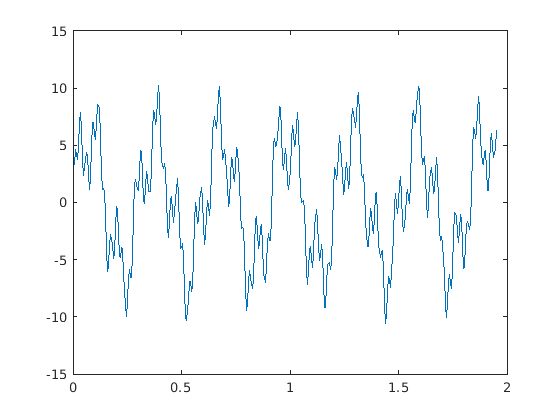
\includegraphics[width=\maxwidth{56.196688409433015em}]{figure_0.png}
\end{center}


\begin{matlabcode}
%% Decompose by parallel EMD
[out0,val0,idx0,len0,up0,low0] = mex_gpuEMD_env(A,nm, nsift);
\end{matlabcode}
\begin{matlaboutput}
Number of IMF = 3
x_len value is 390, y_len is 203
Running parallele EMD on GPU .................................................
> GPU EMD completed
\end{matlaboutput}
\begin{matlabcode}
% Reshpe the output
% %the IMFs should be matrices with the same shape as A
out = reshape(out0, x_len, y_len, nm);
val = reshape(val0, x_len*2, y_len, nm);
idx = reshape(idx0, x_len*2, y_len, nm);
len = reshape(len0, y_len, nm);
up = reshape(up0, x_len, y_len, nm);
low = reshape(low0, x_len, y_len, nm);

\end{matlabcode}


\begin{matlabcode}
%%
% plot the input and output
figure;
hold off;
subplot(nm+1,1,1);
plot(A(:,1),'k','LineWidth',2);
hold on;
plot(sum(out(:,1,:),3),'r','LineWidth',1);
legend('Input signal','Sum of all IMFs')
yi = 1;
for i = 1:nm
    subplot(nm+1,1,i+1);
    plot(x0(:,i),'DisplayName',['Sinusoid' num2str(i)]);
    hold on;
    plot(out(:,yi,i),'DisplayName',['IMF ' num2str(i)]);
    plot(up(:,yi,i),'DisplayName','Inst. amp');
    %plot(low(:,yi,i));
    plot(idx(1:len(yi,i),yi,i)+1,val(1:len(yi,i),yi,i),'o','DisplayName','cpts');
    legend()
end
\end{matlabcode}
\begin{center}
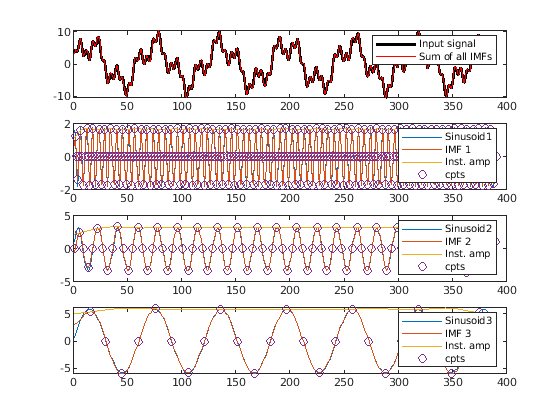
\includegraphics[width=\maxwidth{56.196688409433015em}]{figure_1.png}
\end{center}



\vspace{1em}
\matlabheading{Example 2: decompose sleep epochs and calcualte time-frequency spectrogram}

\begin{par}
\begin{flushleft}
In this example, we cut the whole-night EEG into segments by epoch, decompose all of the epochs at once, and use the output to calcualte  "EMD" styled powerspectrum for each epoch. Then, combining all epochs, we derived the time-frequency representation of EEG by the "EMD" way.
\end{flushleft}
\end{par}

\matlabheadingthree{Reshape the whole night EEG}

\begin{par}
\hfill \break
\end{par}

\begin{matlabcode}
% Reshape the whole-night EEG
EEGA = buffer(EEG, epochL);
% Decompose by parallel EMD
nm = floor(log2(epochL/2));
nsift = 10;

[out0,val0,idx0,len0,up0,low0] = mex_gpuEMD_env(EEGA,nm, nsift);

% Reshpe the output
% %the IMFs should be matrices with the same shape as A
x_len = epochL; y_len = size(EEGA,2); 
out = reshape(out0, x_len, y_len, nm);
val = reshape(val0, x_len*2, y_len, nm);
idx = reshape(idx0, x_len*2, y_len, nm);
len = reshape(len0, y_len, nm);
up = reshape(up0, x_len, y_len, nm);
low = reshape(low0, x_len, y_len, nm);

\end{matlabcode}


\begin{matlabcode}
% Note that the second dimention (y_len) represents the epochs
% Then,with these criticle points and upper envelop, we can define
% power-spectrum the in EMD way
    % calculate insFreq
    InsFreq1 = instFreq3(criticalPoints, epochL, fs, len(iwin,:));
    [fscale,sPowerPlot,~] = freqPowerPlot3(InsFreq1, upperEnv);
% Finally, we plot the time-frequency spectrogram corresponding to sleep
% hypnogram
figure;
subplot(3,1,1); plot(time_hr, sleepscoring.stageNum(1:Nepoch));
xlim([0,time_hr(end)]);
ylabel('Sleep stage')
subplot(3,1,2:3); imagesc(time_hr,fscale,timePowerPlot(10:end,1:Nepoch).^0.25);
axis xy
ylim([0, 30])
ylabel('frequency'); xlabel('Time (hr)')
\end{matlabcode}
\begin{center}
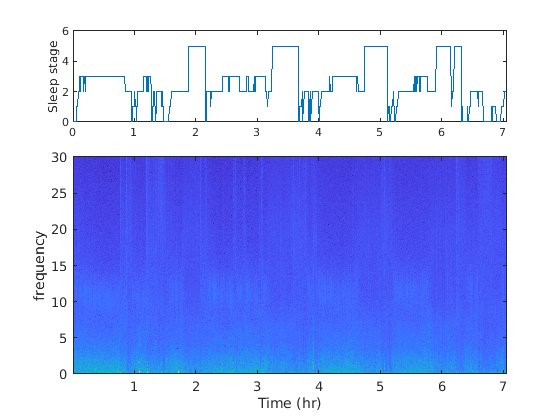
\includegraphics[width=\maxwidth{56.196688409433015em}]{figure_2.png}
\end{center}


\matlabheading{Speed test}

\begin{matlabcode}






\end{matlabcode}

\end{document}
